\section{Montagens e densidade em espaços de funções contínuas}
\label{sec:assemblies}

\begin{definition}[montagem contínua]\label{def:assembly}
Se $K=[\alpha,\beta]$ é um intervalo compacto não degenerado, $\Aclass(K)$ é o conjunto das funções $g\in C(K)$ para as quais existe uma coleção finita $\Lambda$ de células diádicas, com interiores disjuntos e união contendo $K$, e endereços $n(J)$, $J\in\Lambda$, tais que
\begin{equation}
 g|_{J\cap K}=\ell_{n(J)}|_{J\cap K},
 \label{eq:assembly}
\end{equation}
com valores coincidentes nas fronteiras compartilhadas.
\end{definition}

Para $f\in C(K)$, denote o módulo de continuidade por
\begin{equation}
 \omega(f;\delta)=\sup\{|f(x)-f(y)|:x,y\in K,\ |x-y|\le\delta\}.
\end{equation}

A densidade por interpolantes afins e a teoria de splines lineares são
clássicas \citep{deboor2001,powell1981,schumaker2007}. O resultado seguinte
registra o ponto adicional necessário aqui: nós diádicos, valores racionais e
inclinações não nulas podem ser impostos simultaneamente.

\begin{theorem}[densidade das montagens]\label{thm:density}
Para todo $f\in C[\alpha,\beta]$ e todo $\varepsilon>0$, existe $g\in\Aclass([\alpha,\beta])$ tal que
\[
 \|f-g\|_{\infty,[\alpha,\beta]}<\varepsilon.
\]
Todas as peças de $g$ pertencem a $\Library$ e têm inclinação não nula.
\end{theorem}

\begin{proof}
Estenda $f$ por constantes: $F(x)=f(\alpha)$ para $x<\alpha$, $F=f$ em $[\alpha,\beta]$ e $F(x)=f(\beta)$ para $x>\beta$. A extensão é uniformemente contínua. Escolha $k$ de modo que, com $h=2^{-k}$,
\begin{equation}
 \omega(F;h)<\varepsilon/2.
 \label{eq:modulus-choice}
\end{equation}
Tome os nós $t_j=jh$ desde $j_{\min}=\lfloor\alpha/h\rfloor$ até $j_{\max}=\lceil\beta/h\rceil$. Para cada $j$, escolha racional $v_j$ com $|v_j-F(t_j)|<\varepsilon/2$ e, sequencialmente, imponha $v_{j+1}\neq v_j$. Isso é possível porque cada intervalo aberto de escolha contém infinitos racionais e apenas um valor é proibido em cada passo.

Seja $g$ o interpolante linear dos pares $(t_j,v_j)$. Em $J_{k,j}$, sua inclinação é $(v_{j+1}-v_j)/h\in\Qstar$ e seu valor no centro é $(v_j+v_{j+1})/2\in\mathbb{Q}$. Pelo \cref{thm:dictionary}, a peça é o único átomo com esses parâmetros. Os valores nodais compartilhados tornam $g$ contínua.

Se $P_kF$ é o interpolante dos valores exatos, então, para $x=(1-\theta)t_j+\theta t_{j+1}$,
\[
 |F(x)-P_kF(x)|
 \le(1-\theta)|F(x)-F(t_j)|+\theta|F(x)-F(t_{j+1})|
 \le\omega(F;h)<\varepsilon/2.
\]
Além disso, $P_kF-g$ é linear em cada célula e seus valores nodais têm módulo menor que $\varepsilon/2$, logo $\|P_kF-g\|_\infty<\varepsilon/2$. A desigualdade triangular conclui.
\end{proof}

O número de células dessa cobertura uniforme é
\begin{equation}
 N_k=\lceil\beta2^k\rceil-\lfloor\alpha2^k\rfloor
     =(\beta-\alpha)2^k+O(1).
 \label{eq:cell-count}
\end{equation}

A \cref{fig:assemblies-pt} mostra duas dessas racionalizações sobre malhas
diádicas e identifica as peças efetivamente pertencentes a $\Library$.

\begin{figure}[t]
 \centering
 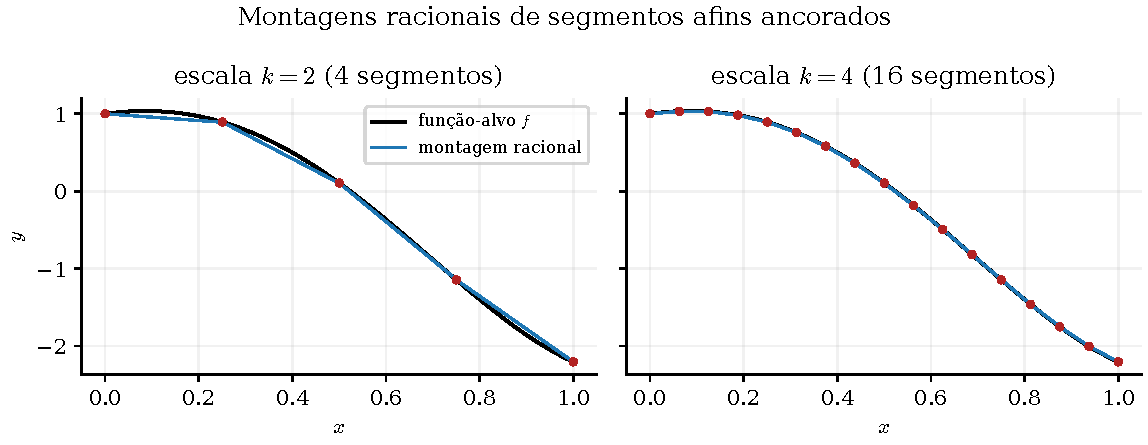
\includegraphics[width=.94\linewidth]{fig03_aproximacao.pdf}
 \caption{Montagens com valores nodais racionalizados em uma grade diádica; cada segmento exibido é um átomo de $\Library$.}
 \label{fig:assemblies-pt}
\end{figure}

\subsection{Equivalência exata com redes ReLU racionais}

Escreva $\rho(z)=z_+=\max\{0,z\}$. A relação entre montagens e redes
lineares por partes pode ser formulada sem aproximação e sem parâmetros reais
ocultos. A identidade em hinges usada a seguir é clássica na representação de
funções lineares por partes por redes ReLU
\citep{yarotsky2017,devorehaninpetrova2021,daubechies2022}; o conteúdo
específico aqui é sua compatibilidade exata com os nós diádicos, os parâmetros
racionais, a recuperação das células e a restrição de inclinação não nula.

\begin{theorem}[equivalência montagem--ReLU racional]
\label{thm:assembly-relu}
Seja $g\in\Aclass(K)$ dada por $N$ folhas consecutivas, com nós
$t_0<t_1<\cdots<t_N$ e inclinação racional não nula $s_j$ em
$[t_j,t_{j+1}]\cap K$, $0\le j<N$. Então, em $K$,
\begin{equation}
 g(x)=g(t_0)+s_0(x-t_0)
      +\sum_{j=1}^{N-1}(s_j-s_{j-1})\rho(x-t_j).
 \label{eq:assembly-relu}
\end{equation}
Depois de expandido o primeiro termo afim, todos os coeficientes são
racionais, todos os pontos de quebra internos são diádicos e
\eqref{eq:assembly-relu} é uma rede ReLU rasa normalizada com $N-1$ unidades
hinge e um termo afim de saída. Unidades cujo peso de saída é zero podem ser
removidas.

Reciprocamente, seja
\begin{equation}
 R(x)=c+qx+\sum_{j=1}^{M}a_j\rho(x-\tau_j),
 \qquad c,q,a_j\in\mathbb Q,\quad \tau_j\in\mathbb D,
 \label{eq:normalized-relu}
\end{equation}
com nós distintos. Suponha que $K$ admita uma cobertura por células diádicas
compatível com os $\tau_j$, que os valores nodais sejam racionais e que cada
inclinação local
\begin{equation}
 q+\sum_{\tau_j<x}a_j
 \label{eq:relu-local-slope}
\end{equation}
seja não nula. Então $R|_K\in\Aclass(K)$. Uma malha diádica uniforme que
refine todos os $\tau_j$ fornece essa montagem explicitamente.
\end{theorem}

\begin{proof}
Na primeira folha, o lado direito de \eqref{eq:assembly-relu} tem valor
$g(t_0)$ em $t_0$ e inclinação $s_0$. Ao atravessar $t_j$, a derivada ganha
exatamente $s_j-s_{j-1}$; por indução, sua inclinação na folha $j$ é $s_j$.
Como ambos os lados são contínuos e coincidem no primeiro nó, coincidem em
todo $K$. Cada $s_j$ é racional. Os nós internos são fronteiras de células
diádicas, e o intercepto do primeiro átomo é racional por
\eqref{eq:global-parameters}; logo a forma expandida tem somente parâmetros
racionais.

Para a recíproca, refine uma grade diádica até que cada $\tau_j$ seja uma
fronteira. Em qualquer célula aberta da grade, \eqref{eq:normalized-relu} é
afim, com inclinação \eqref{eq:relu-local-slope}. O valor no centro da célula
é racional, pois o centro, os nós e todos os coeficientes são racionais. A
hipótese de inclinação não nula permite aplicar o
\cref{thm:dictionary}, que fornece um único átomo da biblioteca nessa célula.
A continuidade de $R$ faz os valores coincidirem nas fronteiras. A união das
peças é, portanto, uma montagem no sentido da \cref{def:assembly}.
\end{proof}

A racionalidade dos valores nodais na recíproca é automática na forma
normalizada \eqref{eq:normalized-relu}; ela foi enunciada separadamente para
deixar explícita a interface exigida de uma parametrização de rede mais geral.
A condição de inclinação não nula não é cosmética: se uma inclinação local
fosse zero, a peça correspondente não teria suporte recuperável pela
\cref{lem:cell-recovery}. Se a arquitetura não oferecer a conexão afim direta,
o termo linear pode ser realizado por
$x=\rho(x)-\rho(-x)$, ao custo de duas unidades adicionais, mantendo o viés
constante na saída.

\begin{proposition}[parâmetros e altura]
\label{prop:relu-complexity}
Na forma normalizada, a conversão de uma montagem com $N$ folhas armazena
$2N$ racionais: o intercepto e a inclinação iniciais, mais um nó e um salto de
inclinação para cada uma das $N-1$ unidades. Se todos os átomos têm altura no
máximo $H\ge2$, a altura máxima dos parâmetros produzidos satisfaz
\begin{equation}
 H_{\mathrm{ReLU}}\le 2^{H+1}H^2.
 \label{eq:relu-height-bound}
\end{equation}
\end{proposition}

\begin{proof}
Há $N-1$ pares $(t_j,s_j-s_{j-1})$, além dos dois parâmetros afins. Pela
definição de altura atômica, $\height(s_j)\le H$, os nós satisfazem
$\height(t_j)\le2^H$, e a forma geral do
\cref{lem:height-arithmetic} dá
$\height(s_j-s_{j-1})\le2H^2$. Para o intercepto inicial, escreva
$a=y_0-sx_0$. Como $\height(x_0)\le2^H$,
\[
 \height(a)\le2\height(y_0)\height(sx_0)
 \le2^{H+1}H^2.
\]
Isso prova \eqref{eq:relu-height-bound}. Como
os demais parâmetros são produtos ou somas dos mesmos dados, essa cota também
garante que a conversão é efetiva em aritmética racional exata.
\end{proof}

O \cref{thm:assembly-relu} estabelece identidade funcional entre montagens e
redes rasas. Os custos de codificação, busca e interpretação constituem
questões distintas. Após fixar códigos prefix-free executáveis, o
\cref{thm:coding-formats} separa o custo de transmitir diádicos como pares
estruturais daquele de expandi-los como frações reduzidas.

A \cref{fig:relu-equivalence-pt} exibe uma instância cujos pesos foram
obtidos pelo mesmo conversor racional exato usado na verificação computacional.

\begin{figure}[t]
 \centering
 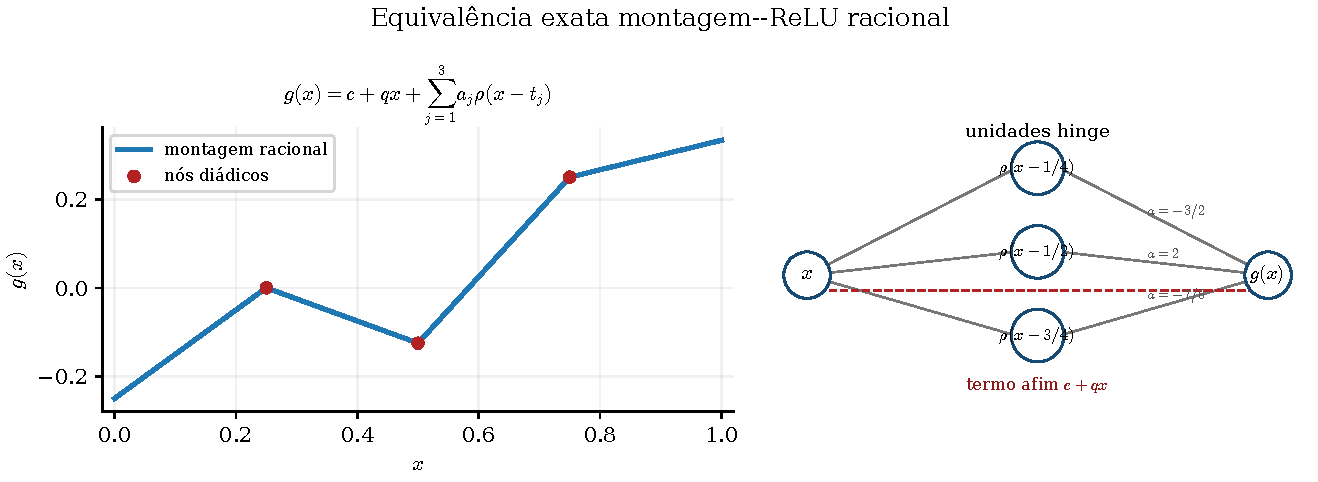
\includegraphics[width=.96\linewidth]{fig07_relu.pdf}
 \caption{Uma montagem racional com quatro folhas e sua rede ReLU rasa
 correspondente. O gráfico e os pesos do diagrama são gerados pelo mesmo
 conversor exato usado nos testes.}
 \label{fig:relu-equivalence-pt}
\end{figure}

\subsection{Relação com o 1-jato de Taylor}

Se $J_{k,m}$ tem centro $x_0$ e largura $h$, o 1-jato de $f\in C^2(J_{k,m})$ é
\[
 T_{x_0}f(x)=f(x_0)+f'(x_0)(x-x_0).
\]

\begin{proposition}[pertencimento e aderência]\label{prop:jet}
Se $f(x_0)\in\mathbb{Q}$ e $f'(x_0)\in\Qstar$, então $T_{x_0}f$ é o átomo de $\Library$ associado à célula. Em geral, para todo $\delta>0$ existem $q_0\in\mathbb{Q}$ e $q_1\in\Qstar$ tais que $\ell_q(x)=q_0+q_1(x-x_0)$ satisfaz
\begin{align}
 \|T_{x_0}f-\ell_q\|_{\infty,J_{k,m}}&<\delta,\label{eq:jet-close}\\
 \|f-\ell_q\|_{\infty,J_{k,m}}&\le \frac{h^2}{8}\|f''\|_{\infty,J_{k,m}}+\delta.
 \label{eq:jet-error}
\end{align}
\end{proposition}

\begin{proof}
No primeiro caso, $(x_0,f(x_0),f'(x_0))$ pertence ao contradomínio do \cref{thm:dictionary}. No caso geral, escolha $q_0$ com $|f(x_0)-q_0|<\delta/2$ e $q_1\neq0$ com $|f'(x_0)-q_1|<\delta/h$. Como $|x-x_0|\le h/2$, obtém-se \eqref{eq:jet-close}. O resto integral de Taylor fornece
\[
 |f(x)-T_{x_0}f(x)|
 =\left|\int_{x_0}^{x}(x-t)f''(t)\dd t\right|
 \le\frac{|x-x_0|^2}{2}\|f''\|_\infty
 \le\frac{h^2}{8}\|f''\|_\infty.
\]
A desigualdade triangular prova \eqref{eq:jet-error}.
\end{proof}

Assim, jatos reais arbitrários pertencem à aderência local da biblioteca racional; não pertencem necessariamente à própria biblioteca.
